\scanpage{99}
\mspage{46}

On aura de $=$, pour $J$ et $L$ quelconques
\[
(109)\qquad
V_{J,L}^Z=
\underset{\substack{d\in\mathrm{Drap}(J\cup L)\\d\cap J\ne\phi,\,d\cap L\ne\phi}}{\unsure{\uline{\lim}|\varinjlim}}
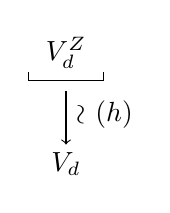
\begin{tikzpicture}[baseline=(top.base),x=1cm,y=1cm]
  \node (top) at (0,0) {$V_d^Z$};
  \draw (-.48,-.25)--(-.48,-.36)--(.48,-.36)--(.48,-.25);
  \draw[->] (0,-.49)--(0,-1.17);
  \node[rotate=90] at (.21,-.79) {$\sim$};
  \node at (.61,-.79) {$(h)$};
  \node at (0,-1.42) {$V_d$};
\end{tikzpicture}
\]
\margin{si $J\prec L$, $J$ et $L$ des bandes et si $Z$ contient $\deleted{X_J^*\unsure{\cap|\cup}}X_L^*$, donc contient $X_{i_n}^*$ si $d=(i_0,\mathord{\cdot}\mathord{-},i_n)$}

\deleted{\unsure{clairement|claire et|claire est}} \inserted{donc si} \inserted{$J,L$ des bandes et $J\prec L$, et si} $Z$ contient $\deleted{X_J^{\unsure{*}}\unsure{\cap|\cup}}X_L^*$, on aura
\[
(110)\qquad V_{J,L}^Z\overset{\overset h{(\sim)}}{\hookrightarrow}V_{\unsure{J|\square},L}
\]
en particulier
\[
(111)\qquad V_{J\unsure{,|0}}^L\left(\overset{\mathrm{déf}}=V_{J,L}^{X_L^*}\right)\overset{\overset h{(\sim)}}{\hookrightarrow}V_{J,L}
\]

Soient
\[
(\unsure{112|111})\qquad J_0\prec J_1\prec \mathord{\cdot}\mathord{-}\prec J_n
\]
des bandes, on posera
\[
(113)\qquad\begin{aligned}
V_{J_0,\mathord{\cdot}\mathord{-},J_n}&=V_{J_0}\cap \mathord{\cdot}\mathord{-}\cap V_{J_n}\\
&=\bigcup_{\substack{j_0\in J_0\\\mathord{\cdot}\mathord{\cdot}\mathord{-}\\j_n\in J_n}}V_{j_0j_1\mathord{\cdot}\mathord{-}j_n}\\
&=\underset{\substack{d\in\mathrm{Drap}(J_0\cup J_1\cup \mathord{\cdot}\mathord{-}\cup J_n)\\d\cap J_0\ne\phi,\mathord{\cdot}\mathord{\cdot}\mathord{-},d\cap J_n\ne\phi}}{\lim_{\longrightarrow}}V_d
\end{aligned}
\]

% This wholly canceled block is upside down relative to the main text. Its reading orientation is restored below; all original positions remain documented in the crop.
\[
\begin{gathered}
\deleted{\unsure{V_J^L}\,\unsure{=}\,\bigcup_{\unsure{j\in J}}V_j\cap X_L^*=}\\
\deleted{\bigcup_{\unsure{l\in L}}{\unsure{V}}_{\unsure{l|L}}^{\unsure{Z|2}}}\\
\deleted{\unsure{\supseteq|\geq}\,\unsure{Z|2}=X_L^*}
\end{gathered}
\]
\margin{98}
